\section{The \computerrl Training}\label{sec:training}
In Section~\ref{sec:framework}, we establish a robust foundation for large-scale agent training. 
However, scaling end-to-end training still faces challenges in initializing a capable base policy and entropy collapse during RL.
This section details our scalable \computerrl training approach and its algorithmic innovations for extended training in desktop environments.

\subsection{Behavior Cloning Setup}\label{sec:bc-training}
To perform a cold start for our model, we employ BC as the initial stage of training. By imitating user interactions, BC enables agents to acquire foundational competencies, thereby facilitating rapid adaptation to computer operations and tasks. 

\vpara{Trajectory Collection with Multiple LLMs.}
We manually collect extensive tasks with corresponding evaluation functions (see Appendix~\ref{apdx:annotation}) and augment to construct an 8k-task dataset.
However, the large-scale collection of high-quality trajectories remains challenging. Manual annotation is prohibitively expensive, and relying on a single model for trajectory generation results in limited and homogeneous data distribution constrained by that model's capabilities.
To address these limitations, we leverage the complementary strengths of multiple advanced models to collect a diverse and high-quality set of interaction trajectories. Concretely, our data pipeline consists of three key stages:

\begin{enumerate}[leftmargin=1.5em,itemsep=0pt,parsep=0.2em,topsep=0.0em,partopsep=0.0em]
    \item \textbf{Initial Sampling}: For each task, we utilize closed-source LLMs to sample several trajectories per task independently. We record both the complete interaction trajectories and the outputs produced by the respective evaluation functions. This procedure yields a rich set of diverse trajectories that serve as the foundation for subsequent data augmentation and model adaptation.

    \item \textbf{Outcome Stratification}: Following initial data collection, we perform a stratified analysis of task outcomes by categorizing all tasks into three groups based on achieved accuracy: \textbf{Fully Solved} ($\mathrm{acc}=100\%$), \textbf{Partially Solved} ($0<\mathrm{acc}<100\%$), and \textbf{Unsolved} ($\mathrm{acc}=0\%$).

    \item \textbf{Task-Oriented Augmentation with Stratified Sampling}: For partially solved tasks, we conduct SFT on our backbone model using the initial trajectories as input. The fine-tuned model is then used to sample additional trajectories for each task, thereby substantially expanding the coverage and quality of trajectories for tasks where model proficiency was previously limited.
    
 For tasks classified as unsolved, we build a model pool of high-performing models and randomly select one to determine each action. This approach leverages inter-model variance at the task level, as different models exhibit distinct areas of expertise despite comparable aggregate performance, enabling trajectory generation that is unattainable by any single model.
\end{enumerate}

\begin{figure}[t]
    \centering
    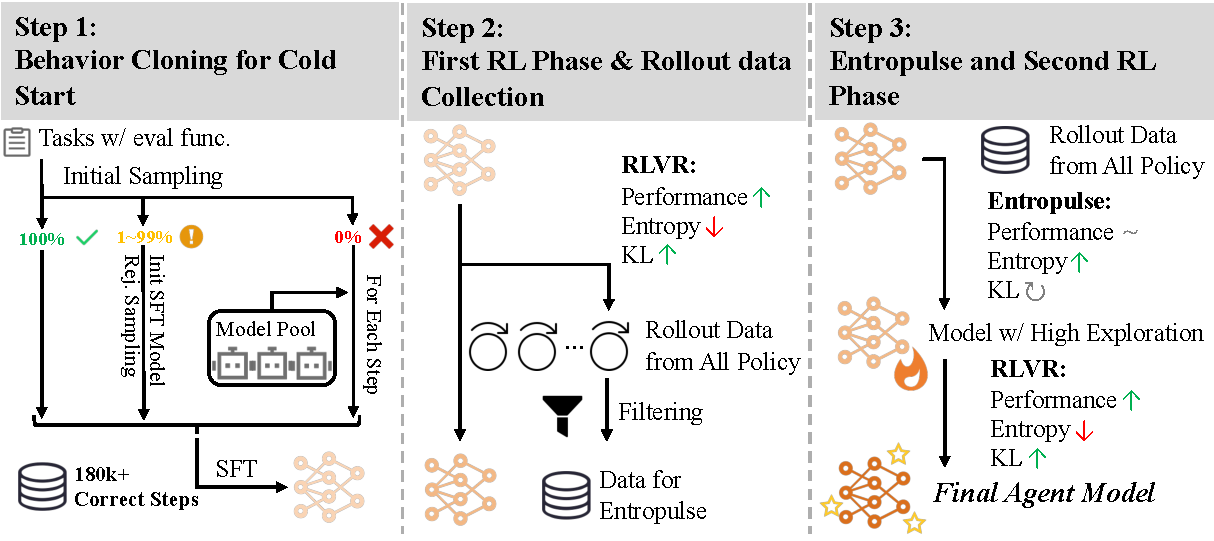
\includegraphics[width=0.95\textwidth]{images/training.pdf}
    \vspace{-1mm}
    \caption{Overview of \computerrl, which includes three stages: (1) BC cold start with trajectories collected from general LLMs; (2) RL with step-level GRPO using verifiable, rule-based rewards; (3) \rlmethod, which alternates RL with SFT on correct rollouts to restore entropy and sustain learning.}
    \vspace{-3mm}
    \label{figs:main}
\end{figure}

We systematically aggregate and filter the collected interaction data, retaining only successful trajectories (\textbf{180k+} correct steps), and employ them for supervised fine-tuning of the model. 
This strategy equips the model with robust desktop manipulation capabilities and foundational reasoning abilities, significantly enhancing the performance of the base model.

\subsection{Reinforcement Learning with Verifiable Rewards}\label{sec:rlvr}

\textbf{Step-Level Group Relative Policy Optimization.}
We extend the GRPO algorithm~\citep{shao2024deepseekmath} to the step-level, making it more suitable for agent RL training. For each task $\tau$, the policy $\pi_{\theta}$ interacts with the desktop environment and samples $G$ trajectories $\mathcal{T}_1, \mathcal{T}_2, \ldots, \mathcal{T}_G$.
The $i$-th trajectory consists of $L_i$ step-level actions $o_{i,1}, \ldots, o_{i,L_i}$.
All steps from the same task are grouped, and the advantage $A_{i,j}$ is computed for each step.
The overall loss aggregates all step advantages as follows:
\begingroup\small
\begin{align*}
\mathcal{J}_{StepGRPO}(\theta) = &\; \mathbb{E}_{\mathcal{T} \sim P(\mathcal{T}), \left\{\{o_{i,j}\}_{j=1}^{L_i}\right\}_{i=1}^{G} \sim \pi_{\theta_{old}}} \Bigg[\frac{1}{\sum_{i=1}^{G} L_i} \sum_{i=1}^{G} \sum_{j=1}^{L_i} \Bigg(\min \Bigg( \frac{\pi_{\theta}(o_{i,j}|q_{i,j})}{\pi_{\theta_{old}}(o_{i,j}|q_{i,j})} A_{i,j}, \\
    & \qquad \text{clip} \Big( \frac{\pi_{\theta}(o_{i,j}|q_{i,j})}{\pi_{\theta_{old}}(o_{i,j}|q_{i,j})}, 1 - \epsilon, 1 + \epsilon \Big) A_{i,j} \Bigg) - \beta \mathbb{D}_{KL}(\pi_{\theta} \| \pi_{ref}) \Bigg) \Bigg],
\end{align*}
\[
A_{i,j} = \frac{r_{i,j} - \text{mean}(\mathcal{R})}{\text{std}(\mathcal{R})}, \quad \mathcal{R} = \{ r_{u,v} \mid u=1,\dots,G, \, v=1,\dots,L_u \}
\]
\endgroup

\textbf{Reward Design.}
We select a subset of the constructed human-annotated data (in Section~\ref{sec:bc-training}) for RL and employ a rule-based verification function to provide verifiable training signals for each trajectory. 
Successfully solved trajectories receive a reward of 1 for every correctly formatted action that contributes to the solution; failed trajectories or improperly formatted actions receive a reward of 0. Unlike conventional approaches that propagate step-wise returns via the Bellman equation, our methodology treats each prompt-response pair as an independent training instance with rewards based on the final trajectory outcome. This direct reward assignment provides explicit feedback by coupling agent behaviors with task success, facilitating effective policy optimization.


\subsection{\rlmethod for Scaling RL Training}\label{sec:rewarm-rl}
In the RL training in Section~\ref{sec:rlvr}, we observe that model performance plateaus after hundreds of training steps, with stagnating task completion rates and decreasing entropy. This premature convergence motivates us to investigate strategies for extending effective training and enhancing policy exploration.
Inspired by DAPO~\citep{yu2025dapo}, we experiment with increasing the clipping threshold, which attenuates the decline in entropy but significantly slows down policy improvement.

To address the issue, we propose \rlmethod, motivated by the observation that SFT and RL objectives differ markedly during training. As entropy decreases during RL optimization, integrating SFT at critical junctures enhances exploration and trajectory diversity, facilitating further policy optimization.
During initial RL training, we aggregate and retain all successful rollout trajectories. While conventionally discarded after single use, these trajectories from various policies at different training steps represent valuable and diverse behavioral data.

We process this dataset by randomly selecting successful trajectories per unique task to construct a new SFT training set, which exhibits the following attributes:
\begin{enumerate}[leftmargin=1.5em,itemsep=0pt,parsep=0.2em,topsep=0.0em,partopsep=0.0em]
    \item \textbf{High quality}: All data comprises completed, high-fidelity trajectories.
    \item \textbf{Diversity}: Rollouts originate from heterogeneous policies in different training steps, offering a variety of problem-solving strategies.
    \item \textbf{Computational efficiency}: The dataset leverages existing interaction data, eliminating the need for additional environment rollouts.
\end{enumerate}

SFT training on this curated dataset produces notable shifts in policy behavior. While evaluation task performance remains stable, the resulting policy shows increased entropy relative to the original one, indicating enhanced exploration.
Building upon this enhanced exploration capability, we conduct a second round of RL training, which yields significant performance improvements and enables us to achieve state-of-the-art results in computer automation.
The training details are in Appendix~\ref{apdx:training_details}.


